\documentclass{amsart}

\usepackage[T1]{fontenc}
\usepackage[utf8]{inputenc}
\usepackage[UKenglish]{babel}
\usepackage{amsmath}
\usepackage{amsthm}
\usepackage{amssymb}
\usepackage{float}
\usepackage{graphicx}
\usepackage{algorithm}
\usepackage{algorithmic}
\usepackage{todonotes}
\usepackage{enumitem}
\usepackage[misc]{ifsym}
\usepackage[foot]{amsaddr}
\usepackage[hidelinks]{hyperref}
\usepackage[style=authoryear,ibidtracker=false,uniquename=false,giveninits=true,terseinits=true,maxbibnames=5,backend=biber]{biblatex}
\renewbibmacro{in:}{}
\addbibresource{lit.bib}

\newcommand{\np}{\mathcal{NP}}
\newcommand{\parent}{\mathrm{parent}}
\newcommand{\mrca}{\mathrm{mrca}}
\newcommand{\rank}{\mathrm{rank}}
\newcommand{\nni}{\mathrm{NNI}}
\newcommand{\rnni}{\mathrm{RNNI}}
\newcommand{\rnniu}{\mathrm{RNNIu}}
\newcommand{\tbr}{\mathrm{TBR}}
\newcommand{\spr}{\mathrm{SPR}}
\newcommand{\csort}{\textsc{Caterpillar Sort}}
\newcommand{\findpath}{\textsc{FindPath}}
\newcommand{\mdtree}{\textsc{MDTree}}

\newtheorem{definition}{Definition}
\newtheorem{theorem}[definition]{Theorem}
\newtheorem{conjecture}[definition]{Conjecture}
\newtheorem{lemma}[definition]{Lemma}
\newtheorem{corollary}[definition]{Corollary}
\newtheorem{proposition}[definition]{Proposition}

\graphicspath{{figures/}}


\title[Ranked Nearest Neighbour Intarchange]{Geometry of Ranked Nearest Neighbour Interchange Space of Phylogenetic Trees}
\date{\today}
\author{Lena Collienne\textsuperscript{1}}
\email{lena.collienne@postgrad.otago.ac.nz}
\address{\textsuperscript{1}Department of Computer Science, University of Otago, New Zealand}
\author{Mareike Fischer\textsuperscript{2}}
\email{email@mareikefischer.de}
\address{\textsuperscript{2}Institute for Mathematics and Inofrmatics, University of Greifswald, Germany}
\author{David Bryant\textsuperscript{3}}
\email{david.bryant@otago.ac.nz}
\address{\textsuperscript{3}Department of Mathematics and Statistics, University of Otago, New Zealand}
\author{Alex Gavryushkin\textsuperscript{1, \Letter}}
\email{\textsuperscript{\Letter}alex@biods.org}


\begin{document}

\maketitle

\begin{abstract}

\end{abstract}

The nearest neighbour interchange ($\nni$) graph, defined on the set of phylogenetic trees with adjacency relation given by the interchange operation of two sister clades, has been known in mathematical biology literature for nearly 50 years \autocite{Robinson1971, Moore-Goodman-Barnabas1973}.
Considered with the metric given by the length of a shortest path (graph-distance), this graph becomes a metric space.
Its geometry has been extensively studied \autocite{...}.
An important property of the $\nni$ graph is that computing distance is NP-hard \autocite{...}.
As a result no algorithm exists to compute the distance in practical time \autocite{...Whidden may be}.
A consequence is that tree search and sampling algorithms pose a significant challenge even for moderately sized trees \autocite{...}.

More recent advances in computational phylogenetics introduce various classes of molecular clock models \autocite{...} and made possible computational inference of phylogenetic time-trees \autocite{...}.
However, mathematical challenges that come with this seemingly inessential change in parametrisation (genomic distance VS time distance) of trees have only recently been brought to attention \autocite{Gavryushkin2016-uu}.
\textcite{Gavryushkin2018-ol} have proposed an extension of the $\nni$ graph to the class of discrete time-trees.
The simplest such extension introduces the $\rnni$ graph on the set of ranked phylogenetic trees.
Considered with the graph-distance $\rnni$ becomes a metric space and inherits the geometric and algorithmic challenges that the $\nni$ space has been traditionally facing.
Surprisingly, most of them cannot be settled by directly translating results or applying techniques developed for $\nni$ \autocite{Gavryushkin2018-ol}.

\todo{LC: mention some results here and how they make $\rnni$ differ from $\nni$}
This distinguishes $\rnni$ from $\nni$ where this does not hold.
One further result, presented in Section~\ref{section:diameter}, directly following from the proof of Theorem~\ref{thm:caterpillar_convex}, is the diameter of $\rnni$.
Finally, we disprove the so-called Strong Split Theorem, conjectured in \autocite{Gavryushkin2018-ol}.
However, the Weak Split Theorem remains a conjecture.
Furthermore, we propose an alternative (even weaker) version of the conjecture, the Cluster Theorem (Section~\ref{section:split_theorem}).



In this paper, we consider the $\rnni$ space on the ranked phylogenetic trees with all taxa being of equal rank.
An example of such a tree is depicted in Figure~\ref{fig:...}.
In the terminology of \autocite{Gavryushkin2018-ol}, the space considered in this paper is the space of ranked ultrametric phylogenetic trees $\rnniu$.
We postpone accurate definitions until later in this section.

[Figure of ranked tree]

In line with the research programme proposed in \autocite{Gavryushkin2018-ol}, we investigate the geometry and algorithmic complexity of the $\rnni$ space.
Specifically, in this paper we establish the exact radius and diameter of the space, [... -- Lena, please finish this including the approaximate algorithm that works exactly on small spaces (Lena: is it already in the text?)]
The question of whether there exists a polynomial algorithm for computing the $\rnni$ distance remains an open problem.

In the rest of this chapter we formally introduce non-standard definitions necessary for this paper.

A \emph{ranked phylogenetic tree} is a pair consisting of a rooted binary phylogenetic tree $T$ on the set $X = \{1, \ldots, n\}$ of \emph{taxa} for $n \in \mathbb N$, and a (total) rank function $\rank$ that maps all elements of $X$ to $0$, all internal nodes of $T$ onto the set $\{1, \ldots, n-1\}$, and respects the partial order given by the tree.
The latter means that if $u$ and $v$ are two internal nodes of $T$ such that there exists a path from a taxon $x \in X$ to the root which first passes through $u$ and then through $v$ then $\rank(u) < \rank(v)$.
Ranked trees $(T_1, \rank_1)$ and $(T_2, \rank_2)$ are different if trees $T_1$ and $T_2$ are different or $T_1 = T_2$ and $\rank_1 \neq \rank_2$.
Since all trees in this paper are ranked trees, we will abuse the notation and drop the ranking from the notation.
We will also refer to a ranked tree simply by tree.
For a tree $T$, we will use $\rank_T$ to refer to its ranking.

Our definition of a ranked tree implies a natural notion of the edge length.
Indeed, a tree edge $(u,v)$ of $T$ has length $l$ if $|\rank_T(v) - \rank_T(u)| = l$.

Now we are ready to define the tree space which is the subject of study in this paper, the $\rnni$ graph.

The vertex set of the $\rnni$ graph is the set of all ranked trees on $n$ taxa.
We introduce two types of operation ($\rnni$ \emph{moves}) on trees (see Figure~\ref{fig:RNNI}) and say that two trees are adjacent in the $\rnni$ graph if they are connected by an operation of either type.
The first type of operation is called a \emph{rank move} and defined by swapping the ranks of two internal nodes that are not adjacent in the tree.
Formally, if $u$ and $v$ are such nodes of a tree $T$ that $|\rank_T(u) - \rank_T(v)| = 1$ and $(u, v)$ is not an edge in $T$ then the tree $R$ obtained from $T$ by only changing $\rank_R(u) = \rank_T(v)$ and $\rank_R(v) = \rank_T(u)$ is said to be obtained by a rank move.
The second type of operation is called an $\nni$ \emph{move} and defined in the usual way, that is, two trees $T$ and $R$ are said to be connected by an $\nni$ move if there exist internal edges $e$ in $T$ and $f$ in $R$ both of length one such that the trees obtained by shrinking $e$ and $f$ to internal nodes coincide.

We use the notation $d(T, R)$ throughout the paper to denote the graph distance between trees in $\rnni$, that is, $d(T, R)$ is the length of a shortest $\rnni$ path between $T$ and $R$.

\todo{Add a bit more space in all figures at the bottom to have at least a standard interval above he caption.}
\todo{In this figure -- rm arrows (think how to place the RNNI edges), possibly avoid using colour, and highlight where the rank move is made (hollow nodes?)}
\todo{Two of these trees are caterpillar trees.
Do you think it would be helpful to draw them as caterpillars to prepare readers for the rest of the paper?}
\begin{figure}[H]
	\centering
	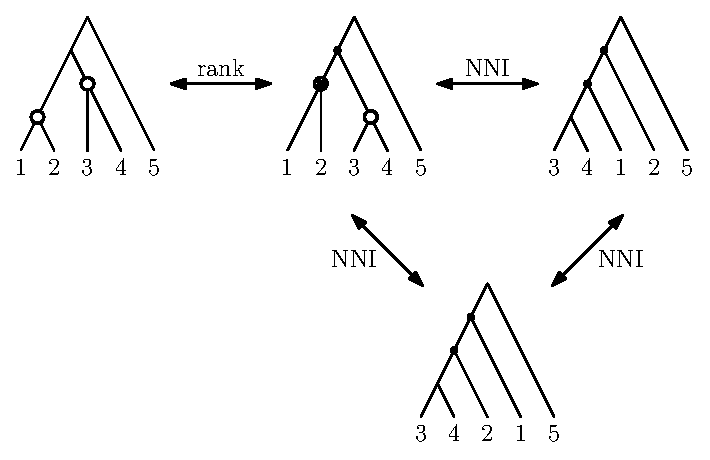
\includegraphics[width=0.8\textwidth]{RNNI}
    \vspace{2pt}
	\caption{Two types of operation that define edges of the $\rnni$ graph.}
	\label{fig:RNNI}
\end{figure}


\todo{LC: Explain structure of paper}


\section{Algorithms}
\label{section:algorithms}

Within this section we will first introduce two algorithms, namely $\findpath$ (Section~\ref{section:alg_findpath}) and $\csort$ (Section~\ref{section:alg_csort}), for computing paths between two given trees in $\rnni$.
The first one takes arbitrary trees as input while the latter one is restricted to trees with a certain tree shape.
We will use them later to prove some geometric properties of the $\rnni$ graph in section~\ref{section:geometry}.
Additionally we will present the algorithm $\mdtree$, which produces a tree that is far away from the given input tree.
What we mean by far away depends on the input tree and will be discussed in Section~\ref{section:alg_mdtree}.


\subsection{$\findpath$}
\label{section:alg_findpath}

Before introducing the algorithm we need the following definitions.
Each node $v$ of a tree defines a \emph{cluster} $C$, which is the set of taxa descending from $v$.
We then say that $v$ \emph{induces} $C$.
\emph{Trivial clusters} are clusters induced by leaves (contain just one element each) and the root of the tree (contains all taxa).
Note that the list of all non-trivial clusters of a tree, sorted according to the rank of the corresponding node, defines the tree unambiguously.
For the rest of this paper we will use the notion cluster and mean non-trivial clusters only because all trees on $n$ taxa share the trivial clusters.

We are now presenting $\findpath$ (Algorithm~\ref{alg:find_path}), an algorithm for computing paths between any two given trees in $\rnni$.
Let $C_1, \ldots, C_{n-2}$ be the clusters of $R$ (the destination tree) where $C_i$ is induced by the node with rank $i$ for $i = 1, \ldots, n-2$.
$\findpath$ computes a path $p$ which initially consists of $T$ only and is extended stepwise.
Let $\hat T$ denote the last tree of $p$ at any point in the algorithm.
For extending $p$, which equals updating $\hat T$, the clusters $C_1, \ldots, C_{n-2}$ are considered in this order.
When arriving at cluster $C_i$ the clusters in $\hat T$ are rearranged by some $\rnni$ moves until $C_i$ is induced by a node in $\hat T$.
This works as follows.
First find the node inducing the smallest cluster containing all elements of $C_k$ in $\hat T$.
This node is denoted by $\mrca_{\hat{T}}(C_k)$ (short for \emph{most recent common ancestor}).
The rank of $\mrca_{\hat{T}}(C_k)$ in $\hat T$ is higher than the rank of the node inducing $C_k$ in $R$, because we consider $C_i$ for increasing $i$.
As a result, all clusters $C_1, \ldots, C_{i-1}$ are induced by some nodes of $\hat T$ as they are in the destination tree $R$.
Now update $\hat{T}$ by performing an $\rnni$ move that decreases the rank of $\mrca_{\hat{T}}(C_i)$.
With Lemma~\ref{lemma:mrca_move} we know that there exists always exactly one $\rnni$ move that decreases the rank of $\mrca_{\hat{T}}(C_i)$.
So we can perform these moves until $\mrca_{\hat{T}}(C_i)$ has the same rank $i$ in $\hat T$ as in $R$.
Repeating this procedure for all clusters of $R$ results in a path from $T$ to $R$.

\begin{algorithm}[H]
\caption{$\findpath$($T,R$)}
\label{alg:find_path}
\begin{algorithmic}[1]
	\STATE $\hat{T} := T$
	\STATE $p := [\hat T]$
	\FOR {$i = 1, \dots, n-2$}
		\STATE Let $C_i$ be the cluster induced by the node with rank $i$ in $R$
		\WHILE {$\rank(\mrca_{\hat{T}}(C_i))>i$}
			\STATE Update $\hat{T}$: Decrease $\rank(\mrca_{\hat{T}}(C_i))$ by an $\rnni$ move \label{alg:line:move_set_down}
			\STATE $p = p+\hat{T}$
		\ENDWHILE
	\ENDFOR
	\RETURN $p$
\end{algorithmic}
\end{algorithm}

%BEGIN: From MareikesVisit

\todo{LC: Work on the following proof! Is it worth introducing intervals for $\rnni$ moves for the proof of the following lemma?}

\begin{lemma}
    Let $T$ be a tree and $C \subset \{1, \ldots, n\}$ a subset of taxa such that $C$ is not induced by any node in $T$.
    There is exactly one tree $T'$ that can be obtained from $T$ by one $\rnni$ move such that $\rank(\mrca_{T'}(C)) = \rank(\mrca_{T}(C)) -1 $.
    \label{lemma:mrca_move}
\end{lemma}

\begin{proof}

    \todo{LC: revise this whole proof}

    Let $(C_1, \ldots, C_n)$ be the list representation of $T$ as introduced above.
    \todo{LC: Introduce this representation above!}
    Let $v:=mrca_T(C)$, let $C_{i+1}$ be the cluster induced by $v$, and let $w$ be the node inducing $C_i$.
    We will distinguish the case that there is an edge $(v,w)$ in $T$ from the case that there is no such edge.

    At first we assume that there is no edge $(v,w)$, which means $C_i \not \subset C_{i+1}$.
    In this case the two sets $C_i, C_{i+1}$ can exchange by a rank swap.
    Since $C \subset C_{i+1}$, this rank swap decreases the rank of $\mrca(C)$ by one and there is no $\nni$ move that could move $\mrca(C)$ down.

    Let us now consider the case that $(v,w)$ is an edge in $T$.
    The only move that could decrease the rank of $\mrca(C)$ is an $\nni$ move on the edge $(v,w)$.
    Let $C_k$ and $C_j$ be the clusters induced by the children of $C_i$.
    Then it is $C_k \cup C_j = C_i$.
    There are two different $\nni$ moves possible on $(v,w)$.
    $C_i$ can either be replaced by $C_j \cup (C_{i+1} \setminus C_i)$ or by $C_k \cup (C_{i+1} \setminus C_i)$.
    To prove that there is always exactly one $\rnni$ moves that decreases the rank of $\mrca(C)$, we need to show that it is either $C \subset (C_j \cup (C_{i+1} \setminus C_i))$ or $C \subset (C_k \cup (C_{i+1} \setminus C_i))$.

    Let $a \in C$.
    Then it is $a \in C_{i+1} = mrca(C)$ and it follows $a \in C_{i+1} \setminus C_i$ or $a \in C_i$.
    If $a \in C_{i+1} \setminus C_i$, $a$ is in the new set after the $\nni$ move.
    So now we will assume that $a \in C_i$.
    Then it is either $a \in C_j$ or $a \in C_k$.
    Without loss of generality we assume that $a \in C_j$.

    We need to prove that if $a \in C_j$, there is no $b \in C$ with $b \in C_k$.
    This makes sure that it is either $C \subset (C_j \cup (C_{i+1} \setminus C_i))$ or $C \subset (C_k \cup (C_{i+1} \setminus C_i))$.
    For contradiction we assume that $a \in C_j$ and $C \in S_k$.
    We know that all sets that are subsets of $C$ already are at the same position in the current tree as in the destination tree $R$.
    Therefore, we can conclude from $a \in C_j$ and $b \in C_k$ that $C_j \cup C_k = C$.
    Hence, it holds $mrca(C) = C_i$.
    This is a contradiction to our assumption that $C_{i+1} = mrca(C)$ in the current tree.
    Therefore, it holds either $C \subset (C_j \cup (C_{i+1} \setminus C_i))$ or $C \subset (C_k \cup (C_{i+1} \setminus C_i))$.

    Concluding, there is always an $\rnni$ move on the edge $(v,w)$ for $mrca(C) = C_{i+1}, C \subsetneq C_{i+1}$ that decreases the rank of $mrca(C)$.

\end{proof}

Since $\findpath$ computes a path between two arbitrary trees in $\rnni$, we can use the length of such a path as approximation for the distance between the trees.
A natural question is now how well this estimates the actual distance in $\rnni$.
To answer this question for small trees, we implemented $\findpath$.
\todo{LC: github - link}
For computing the actual $\rnni$ distances we used the the algorithm for computing the $\rnni$ graph that was introduced in Section 3.3 of \autocite{Gavryushkin2018-ol}.
With our implementation of this algorithm
\todo{LC: gihub - link}
we can compute the graph for trees with up to $8$ taxa in reasonable time. \todo{LC: Shall we say more about the algorithm here? + running time (in hours/minutes) on which computer?}
We used
\todo{LC: How do we compare the distances?}

The running time of $\findpath$, implemented as described by the pseudo-code in Algorithm~\ref{alg:find_path}, is quadratic in the number of taxa.
\todo{LC: Where do we mention the running time?}


\subsection{$\csort$}
\label{section:alg_csort}

\todo{LC: move definitions of caterpillar stuff here}
\todo{LC: pseudo code}

Before introducing an algorithm for computing paths between caterpillar trees, we need to introduce further notations.
We aim to find paths between \emph{caterpillar trees} where each internal node has at least one child that is a leaf.
A path $p$ between two caterpillar trees $T$ and $R$ that only consists of caterpillar trees is called \emph{caterpillar path}.
If $p$ is shortest among all caterpillar paths between these trees we call it \emph{shortest caterpillar path}, and the length of $p$ will be denoted by $d_c(T,R)$ and called \emph{caterpillar distance}.

We next introduce a representation of caterpillar trees as lists of taxa.
We will use it to show how one can adapt the classical \emph{Bubble Sort} algorithm \autocite{Knuth1997-pi} to compute caterpillar paths.
\todo{LC: pseudo-code}
Ordering the taxa of a caterpillar trees as a non-decreasing, according to the ranks of their parents, gives us a list of length $n$.
Note that the only two elements in such a list that have parents of equal rank are the first two elements $c_1$ and $c_2$.
We will call a pair of two taxa that share their parent \emph{cherry}.
\todo{LC: pair of taxa or subtree (includes internal node and two edges)}
To make the list representation of caterpillar trees unique, we assume that it is $c_1 < c_2$ for the first two elements in the list.

In the following we explain how $\rnni$ moves between caterpillar trees work in the list representation.
At first it is important to realise that the only possible $\rnni$ moves between caterpillar trees are $\nni$ moves, since there is no pair of internal nodes with rank difference one that is not connected by an edge.
$\nni$ moves between caterpillar trees correspond to swaps of two neighboured elements in the list representation.
The only exception of this are $\nni$ moves on the lowest internal edge, that is the edge connecting the internal nodes of rank one and two.
There are two $\nni$ moves possible on this edge that result in caterpillar trees, while there is for every other edge only one $\nni$ move that results in a caterpillar tree.
Corresponding to the $\nni$ moves on the lowest internal edge are exchanges of either the first or the second element with the third elements in the list representation.

For computing shortest caterpillar paths we modify Bubble Sort as described in the following.
We call this algorithm $\csort$ (Algorithm~\ref{alg:csort}).

\todo{Description + Pseudo code $\csort$}
We consider the input trees $T$ and $R$ in their list representation $L_T$ and $L_R$ as described above and want to compute a path from $L_T$ to $L_R$.
A path $p$ is built stepwise by adding a new list to the end of $p$.
We call the last element of $p$ at any step $L_{\hat T}$ and when we say we update $L_{\hat T}$, we modify this list and append the new version of $L_{\hat T}$ to $p$.

As in the Bubble Sort algorithm, we go through the list $L_{\hat T}$ and swap two elements if they appear in different orders in $L_{\hat T}$ and $L_R$.
Each swap of elements is an update of $\hat T$ and extends the path $p$ by one element.
We compare pairs of list elements from the start of the list until its end, and repeat this until the whole list is sorted, just as in classical Bubble Sort.
Our algorithm $\csort$ only differs from Bubble Sort when considering the first three elements of the list.
Since the first two elements refer to the cherry taxa of the caterpillar tree, both can exchange with the third element of the list as $\nni$ move.
Therefore, we need to consider these moves separately to all other moves.
Most importantly, we need to make sure that these moves are performed in a way that leads to a shortest caterpillar path.
We can guarantee this, if the moves are done as described in the following.
Let $c_1, c_2$ and $c_3$ be the first three elements of $L_{\hat T}$, in this order.
If $c_1$ ($c_2$) is the last element of those three in $L_R$, we update $L_{\hat T}$ by swapping $c_1$ ($c_2$) and $c_3$.
By doing this we make sure that there will be no point on $p$ where $c_1$ and $c_2$ swap positions, which would cause an additional $\nni$ move that can be avoided if we perform the moves as we describe them here.

Because all moves between caterpillar trees are $\nni$ moves as described in the previous paragraph, all pairs of taxa that are not in the same order in $L_T$ and $L_R$ need to swap at some point on any path between $L_T$ and $L_R$.
And since only elements that are direct neighbours in a sequence are allowed to swap, with the only exception being the first three elements, the path computed by $\csort$ is a shortest caterpillar path.
\todo{LC: Do we need further explanation why $\csort$ gives a shortest caterpillar path?}

\todo{LC: improve readability of pseudo-code}

\begin{algorithm}[H]
\caption{$\csort$($T,R$)}
\label{alg:csort}
\begin{algorithmic}[1]
    \STATE $\hat T:= T$, $p = [\hat T]$
    \STATE $L:=$ list representation of $\hat T$
	% \STATE $L_{\hat T} :=$ list representation of $\hat T$, $L_R :=$ list representation of $R$
    \FOR {$i=0,\ldots,n-1$}
        \STATE $j = 0$ \COMMENT{Special case: cherry}
        \IF {$L[0]$ is last element of $L[0],L[1],L[2]$ in list representation $R$}
            \STATE Update $\hat T$: swap $L[0]$ and $L[2]$
        \ELSIF {$L[1]$ is last element of $L[0],L[1],L[2]$ in list representation $R$}
            \STATE Update $\hat T$: swap $L[1]$ and $L[2]$
        \ENDIF
        \STATE $j = 2$
	    % \IF {$L_R^{-1}[L_{\hat T}[j]] > L_R^{-1}[L_{\hat T}[j+1]]$}
        \IF {order of $L[j]$ and $L[j+1]$ different in $\hat T$ and $R$}
			\STATE Update $\hat{T}$: Swap $L[j+1]$ and $L[j]$
			\STATE $p = p+\hat{T}$
		\ENDIF
    \ENDFOR
	\RETURN $p$
\end{algorithmic}
\end{algorithm}

\todo{Check throughout that $\parent$ is never used without tree name in the index.}


\subsection{$\mdtree$}
\label{section:alg_mdtree}

The algorithm we are going to introduce here will be important for finding the radius of the $\rnni$ graph.
In Section~\ref{section:diameter} we will prove that it computes a tree with maximum distance from a given caterpillar tree, which implies that the radius of $\rnni$ equals its diameter.
Therefore, it is called $\mdtree$ (Maximum Distance Tree).
\todo{LC: References to the corresponding proofs?}

$\mdtree$ works as follows for an input tree $T$:
At first, all taxa of $T$ are sorted in a list $L$ such that the ranks of their parents are non-decreasing.
If the input is a caterpillar tree, it follows that $L[0]$ and $L[1]$ are the cherry taxa of $T$, in an arbitrary order, and $\parent(L[i])$ has rank $i$ in $T$ for all $i = 2, \ldots, n-1$.
Note that this list $L$ does not give a unique representation of a tree.
The output tree $R$ is built inductively as follows:
Initially, $R$ only consists of a cherry with taxa $L[0]$ and $L[1]$ such that the parent of these taxa has rank $n-1$.
All following taxa in $L$ are added to $R$ sequentially, according to their order in $L$, by creating a new internal node at one of the existing branches in $R$ such that this new node has rank one less than the previously lowest internal node in $R$.

Algorithm~\ref{alg:max_dist_tree} provides the pseudocode for this algorithm.
We will see in Section~\ref{section:diameter} that it computes trees with maximum distance form any given caterpillar tree.
But if the given tree is an arbitrary tree, the output tree might not have maximum distance to the input tree.

\todo{LC: Shall we give an example where the distance is not max or simulate trees and compute histogram of distances approximated by $\findpath$?}

\begin{algorithm}[H]
\caption{$\mdtree(T)$}
\label{alg:max_dist_tree}
\begin{algorithmic}[1]
	\STATE $R$ only contains cherry taxa $a, b$ of $T$ and has internal node with rank $n-1$
    \STATE In list $L$ all taxa $\{1,\ldots,n\}\setminus\{a,b\}$ are ordered such that the ranks of their parents in $T$ do not decrease
	\FOR {taxon $a$ in $L$}
		\STATE Add an internal node as parent of $a$ on an edge in $R$ such that the new internal node has rank one less than the previously lowest internal node
	\ENDFOR
	\RETURN $R$
\end{algorithmic}
\end{algorithm}



\section{Geometry of $\rnni$}
\label{section:geometry}

In this section we analyse shortest paths in $\rnni$.
Therefore, we will use the algorithms introduced in the previous section.
They enable us to prove that there is always a shortest path between two caterpillar trees that only consists of caterpillar trees (Theorem~\ref{thm:caterpillar_convex}) in Section~\ref{section:caterpillar_convex}.
In other words, the set of caterpillar trees is \emph{convex} in $\rnni$.

This algorithm gives an upper bound for the diameter of $\rnni$, which
\todo{Why is that?}
improves
the one given in \autocite{Gavryushkin2018-ol}.
\todo{When}
Later we will see that this bound is tight.
However, we don't know how good $\findpath$ approximates distances in $\rnni$. \todo{Can we say something about the approximation ratio?}

\todo{make sure trees are consistently denoted by upper case letters}
\begin{lemma}
$\Delta(\rnni) \leq \frac{(n-1)(n-2)}{2}$, where $\Delta(\rnni)$ denotes the diameter of the $\rnni$ graph, that is, if $d(T, R)$ is the graph distance in $\rnni$ then $\Delta(\rnni) = \max \{d(T, R) \mid T, R \in \rnni\}$.
\label{lemma:diameter_bound}
\end{lemma}

\begin{proof}
Since the diameter is bounded from above the maximum length of a path computed by $\findpath$, it is enough to find this maximum.
The worst-case execution of $\findpath$ would require each of the $n-2$ clusters $C$ induced by internal nodes of $R$ to be moved by $n - 1 - i$ $\rnni$ operations in $\hat{T}$.
Hence, the maximum length of such a path is bounded by $\sum\limits_{i = 1}^{n-2} i = \frac{(n-2)(n-1)}{2}$.
\end{proof}

The following lemma relates distances between trees on $n$ and $n+1$ taxa and is an important tool for inductive arguments.
We use the notion $\parent_T(x)$ to refer to the node adjacent to taxon $x$ in tree $T$.
$T{\big|}_n$ denotes the restriction of tree $T$ to the set of taxa $\{1, \ldots, n\}$.
In particular if $T$ is a tree on taxa $1, \ldots, n+1$ the tree $T{\big|}_n$ is obtained by deleting taxon $n+1$ and suppressing the thereby created node of degree two.

\begin{lemma}
Let $T$ and $R$ be two trees on taxa $\{1, \ldots, n+1\}$.
Then $d(T{\big|}_n, R{\big|}_n) \leq d(T,R) - \delta$, where $\delta = |\rank_T(\parent_T(n+1)) - \rank_R(\parent_R(n+1))|$.
\label{lemma:distance_delete_taxon}
\end{lemma}

\begin{proof}
First observe that the rank of an internal node $v$ of a tree $T$ along an $\rnni$ path $p$ can only be changed by performing a rank move that involves $v$ or an $\nni$ move on an edge adjacent to $v$.
Second observe that any $\rnni$ move can change the rank of an internal node by at most one.

Let $p$ be a shortest path from tree $T$ to $R$ and $p{\big|}_n$ the path resulting from deleting taxon $n+1$ from all trees on $p$.
This new path $p{\big|}_n$ is then a path from $T{\big|}_n$ to $R{\big|}_n$.
Recall that $\delta$ is the difference in ranks between the parents of taxon $n+1$ in $T$ and $R$.
\todo{This statement has to be checked very carefully and one or two sentences added to explain the `applying'.}
Applying the two observations above we conclude that $|p{\big|}_n| \leq |p| - \delta$.
Since $d(T{\big|}_n,R{\big|}_n) \leq |p{\big|}_n|$ and $|p| = d(T,R)$, the desired inequality follows.
\end{proof}

Using the same argument as in the proof of Lemma~\ref{lemma:distance_delete_taxon} we can establish the following Proposition~\ref{proposition:lower_bound_distance} that provides a lower bound on the distance between trees.

\begin{proposition}
If trees $T$ and $R$ and taxon $x$ are such that $|\rank_T(\parent_T(x)) - \rank_R(\parent_R(x))| = \delta$ then $d(T,R) \geq \delta$.
\label{proposition:lower_bound_distance}
\end{proposition}


\subsection{The set of caterpillar trees}
\label{section:caterpillar_convex}

In this section we restrict our attention to the set of \emph{caterpillar trees} where each internal node has at least one child that is a leaf.
This type of tree is of particular interest in $\rnni$ because shortest paths between such trees in $\rnni$ differ from those in classical $\nni$ space.
This in combination with the importance of caterpillar trees in the proof of $\np$-hardness of $\nni$ distances in \autocite{Dasgupta2000-xa} suggests that understanding the geometry of paths between caterpillar trees helps investigating the complexity of computing $\rnni$ distances.
In particular, we are going to prove that one can always find a shortest path between two caterpillar trees that contains caterpillar trees only, meaning that the set of caterpillar trees is convex in $\rnni$.
We discovered this by computing caterpillar paths using an algorithm to compute shortest paths within the set of caterpillar trees and comparing them with shortest path in $\rnni$.
This algorithm will be explained in detail later in this section, after demonstrating why finding shortest paths between caterpillar trees builds the basis for understanding the difference between $\nni$ and $\rnni$.


We now compare shortest paths between caterpillar trees in $\nni$ with those in $\rnni$.
In $\nni$, building a cherry and moving it may give a path that is shorter than a path where the taxa move separately in as it is illustrated out in Figure~\ref{fig:NNI_vs_RNNI}.
There is only one move needed to build and resolve a cherry, respectively, while the number of moves for moving the cherry is the same as for moving a single taxon in $\nni$.
But in $\rnni$ space there are additional rank moves needed to change the rank of the internal node of the cherry before an $\nni$ move resolves it.
This is due to the fact that $\nni$ moves are only allowed on edges of length one in $\rnni$.
Therefore, a path where taxa move separately and no second cherry is built, is shortest in $\rnni$.

\begin{figure}[H]
	\centering
	\includegraphics[width=\textwidth]{NNI_vs_RNNI}
	\caption{Paths between caterpillar trees $T$ and $R$: black -- shortest path in classical $\nni$ (ignoring ranks) of length $5$; red -- shortest path in $\rnni$ of length $6$; blue -- path in $\rnni$ which is the natural extension of the shortest path in $\nni$ but has length $8$.}
	\label{fig:NNI_vs_RNNI}
\end{figure}

The above observation suggests that there is always a caterpillar path that is shortest path between two arbitrary caterpillar trees in $\rnni$.
Indeed, we are going to prove Theorem~\ref{thm:caterpillar_convex} within this section, which states that the set of caterpillar trees is convex in $\rnni$.
Note that this is not true for the $\nni$ space, which is clear from the example in Figure~\ref{fig:NNI_vs_RNNI}.


Lemma~\ref{lemma:caterpillar_dist=diameter} regards caterpillar trees with distance $\frac{(n-1)(n-2)}{2}$ and will be needed for proving the convexity of the set of caterpillar trees in $\rnni$.
Notice that we by Lemma~\ref{lemma:diameter_bound} $\frac{(n-1)(n-2)}{2}$ is the upper bound for the diameter of $\rnni$.

\begin{lemma}
    Let $T$ and $R$ be two caterpillar trees.
    $T$ and $R$ have distance $d(T,R) = \frac{(n-1)(n-2)}{2}$ if, and only if, they have caterpillar distance $d_c(T,R) = \frac{(n-1)(n-2)}{2}$.
    \label{lemma:caterpillar_dist=diameter}
\end{lemma}

\begin{proof}
    Let $T$ and $R$ be caterpillar trees.
    Let us first prove that if $d(T,R) = \frac{(n-1)(n-2)}{2}$, it follows $d_c(T,R) = \frac{(n-1)(n-2)}{2}$.
    This easily follows from algorithm $\csort$:
    In each loop $i=1, \ldots, n-2$ of the algorithm there can be at most $n-1-i$ exchanges of taxa.
    It follows that the maximum length of a path computed by this algorithm is $\sum\limits_{k=1}^{n-2} k = \frac{(n-1)(n-2)}{2}$.
    Since there cannot be a caterpillar path shorter than $\frac{(n-1)(n-2)}{2}$ if it is $d(T,R) = \frac{(n-1)(n-2)}{2}$, it follows $d_c(T,R) =  \frac{(n-1)(n-2)}{2}$.

    For proving the other direction of the statement, let now $T$ and $R$ have caterpillar distance $d_c(T,R) =  \frac{(n-1)(n-2)}{2}$.
    We prove $d(T,R) = \frac{(n-1)(n-2)}{2}$ by induction on the number of taxa $n$ of $T$ and $R$:
    Without loss of generality we can assume that $T$ is the caterpillar tree $(\ldots ((1,2),3), \ldots, n)$ or $(\ldots ((1,2),3), \ldots, n+1)$ in the induction step.
    Let $R$ be a caterpillar tree with distance $\frac{(n-1)(n-2)}{2}$ to $T$.

    Induction basis: $n=3$\\
    There are three trees on $3$ taxa that have distance $1$ from another and are caterpillar trees.
    Hence it is $d(T,R) = d_c(T,R) = 1$ for all pairs of trees $T,R$ on $n=3$ taxa.

    Induction step: $n \to n+1$\\
    Induction hypothesis: For trees $T, R$ on $n$ taxa it is $d(T, R) = \frac{(n-1)(n-2)}{2}$.\\
    Let $T, R$ be trees on $n+1$ taxa with caterpillar distance $\frac{n(n-1)}{2}$.
    Therefore, each of the $\frac{n(n-1)}{2}$ pairs of taxa that is considered when running $\csort$ to compute a path $p$ from $R$ to $T$ exchanges.
    From this we can conclude that taxon $n+1$, whose parent has highest rank in $T$, is part of the cherry of $R$. \todo{Do we need to explain this further (figure)?}
    Let us consider the trees $T{\big|}_n$ to $R{\big|}_n$ that result from $T$ and $R$ by deleting taxon $n+1$.
    $\csort$ computes a path from $T{\big|}_n$ to $R{\big|}_n$ that contains the same exchanges of taxa as $p$, except for the $n-1$ ones on $p$ that involve taxon $n+1$.
    Hence, the caterpillar distance is $d_c(T{\big|}_n, R{\big|}_n) = \frac{n(n-1)}{2} - (n-1)$ = $\frac{(n-1)(n-2)}{2}$.
    So we can apply the induction hypothesis on $T{\big|}_n$ and $R{\big|}_n$ and know that $d(T{\big|}_n,R{\big|}_n) = \frac{(n-1)(n-2)}{2}$.

    According to Lemma~\ref{lemma:distance_delete_taxon}, the distance between $T{\big|}_n$ and $R{\big|}_n$ is at least $d(T{\big|}_n, R{\big|}_n) \leq d(T,R) - |\rank_T(\parent(n+1)) - \rank_R(\parent(n+1))|$.
    We also know $|\rank_T(\parent(n+1)) - \rank_R(\parent(n+1))| = n-1$.
    Suppose, contrary to our claim, that there is a path from $T$ to $R$ of length less than $\frac{n(n-1)}{2}$.
    By the above, it follows that $d(T{\big|}_n, R{\big|}_n) \leq d(T,R) - |\rank_T(\parent(n+1)) - \rank_R(\parent(n+1))| < \frac{n(n-1)}{2} - (n-1) < \frac{(n-1)(n-2)}{2}$.
    Since this is a contradiction to $d(T{\big|}_n, R{\big|}_n) = \frac{(n-1)(n-2)}{2}$, it is proven that $d(T,R) = \frac{n(n-1)}{2} $.
\end{proof}

\begin{theorem}
    The set of caterpillar trees is convex.
    \label{thm:caterpillar_convex}
\end{theorem}

\begin{proof}
    We prove this Theorem by backwards induction on the length $l$ of a shortest caterpillar path between two caterpillar trees $T$ and $R$.
    Since we use backwards induction, we need to consider the maximum distance between any two caterpillar trees as base case, which is $\frac{(n-1)(n-2)}{2}$ as we saw above.

    Induction basis: $l = \frac{(n-1)(n-2)}{2}$\\
    With Lemma~\ref{lemma:caterpillar_dist=diameter} one can see that for each pair of caterpillar trees $T$, $R$ with caterpillar distance $d_c(T,R) = \frac{(n-1)(n-2)}{2}$, it is $d(T,R) = d_c(T,R)$.
    Therefore, there is a shortest path between $T$ and $R$ that is a caterpillar path.

    Induction step: $l+1 \to l$\\
    Induction hypothesis: For each pair of caterpillar trees with caterpillar distance $l+1$ there is a shortest path between these trees that only consists of caterpillar trees, which means that the distance between these trees is $l+1$.
    Let $T$ and $R$ be caterpillar trees with caterpillar distance $l$.
    We consider the shortest caterpillar path computed by $\csort$.
    Since $l < \frac{(n-1)(n-2)}{2}$, there is one loop $k$ when running $\csort$ where less than $n-2-k$ taxon pairs swap positions.
    We assume that this loop number $k$ is the first one in which this occurs.
    This situation is illustrated in the top of Figure~\ref{fig:cat_convex_seq_example}.
    Whenever the number of swaps of taxa or, in terms of sequences, neighboured elements in the sequence is maximum in a loop, one of the two first elements swaps position with $n-2-k$ subsequent elements of the sequence.
    Since we assume that the number of swaps in loop $k$ is not maximal, this does not happen.
    Let us assume that $a$ is the first element that is compared with its left neighbour in loop $k$ but does not swap with it.
    Then the left neighbour $b$ of $a$ in $T$ is below $a$ in $R$ as well.
    Therefore, the tree $T'$ which can be received from $T$ by exchanging $a$ and $b$ must have caterpillar distance $d_c(T',R) = d_c(T,R) + 1 = l + 1$ to $R$.
    For an illustration of the $k^{th}$ loop when performing $\csort$ between $T$ and $R$ or $T'$ and $R$, respectively, consider Figure~\ref{fig:cat_convex_seq_example}.

    \begin{figure}[H]
    	\centering
    	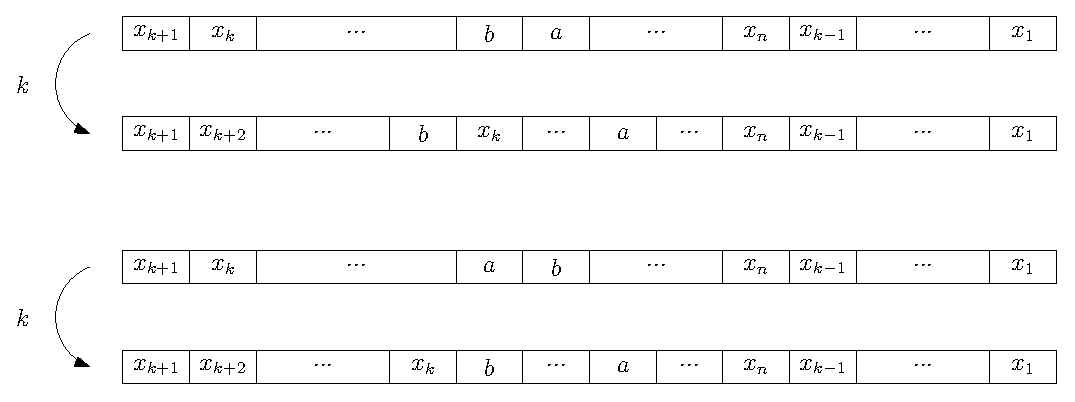
\includegraphics[width=\textwidth]{cat_convex_seq_example}
    	\caption{Loop number $k$ of $\csort$ between $T$ and $R$ as described in proof of Theorem~\ref{thm:caterpillar_convex}.
        The trees are represented as sequences that are being ordered by $\csort$.
        Right before loop number $k$, $x_1, \ldots, x_{k-1}$ are already at the same position as in $R$.
        At the top: sequences between $T$ and $R$ -- $x_k$ and $b$ swap in loop number $k$, but $x_k$ and $a$ not.
        At the bottom: sequences between $T'$ and $R$ -- $a$ and $b$ swap in loop number $k$; $x_k$ and $b$ will swap later}
    	\label{fig:cat_convex_seq_example}
    \end{figure}

    Since it is clear that $T'$ has caterpillar distance $d_c(T',R) = l+1$ to $T$, we can apply the induction hypothesis on $T'$ and $R$ and see that $d(T',R) = l+1$.
    Furthermore, it is $d(T,T') = 1$.
    If it now were $d(T,R) < l$, it would hold $d(T',R) \leq d(T,R) + d(T,T') < l + 1$ which contradicts the induction hypothesis.
    We can conclude $d(T,R) = l$, which completes the proof.
\end{proof}


\subsection{Diameter and radius}
\label{section:diameter}

With the results of Section~\ref{section:caterpillar_convex} we can easily provide the exact diameter of the $\rnni$ graph and hence improve the bounds for the diameter given in \autocite{Gavryushkin2018-ol}.
Furthermore, we are able to show that the \emph{radius} of the $\rnni$ graph, which is defined as $rad(G) =  \min\limits_u \max\limits_v d(u,v)$ for a graph $G$, equals its diameter.
Let us first consider the diameter of the $\rnni$ graph.
With the results of Section~\ref{section:caterpillar_convex} is not hard to see that is $\Delta(\rnni) = \frac{(n-1)(n-2))}{2}$ as it is stated in Corollary~\ref{corollary:diameter}.

\begin{lemma}
	There are two caterpillar trees in $\rnniu$ with distance $\frac{(n-1)(n-2)}{2}$.
	\label{lemma:caterpillar_diameter}
\end{lemma}

\begin{proof}
	Let $T = (( \dots (n,1)2)\dots)n-1)$ and $R = (( \dots (n,n-1)n-2)\dots)1)$.
    According to Theorem~\ref{thm:caterpillar_convex}, there is a shortest path between $T$ and $R$ that is a caterpillar path.
    We can compute a shortest caterpillar path by using $\csort$ as explained in Section~\ref{section:caterpillar_convex}.
    When running this algorithm on $T$ and $R$, each taxon $i$ ($i \in \{1, \ldots, n\}$) swaps $n-1-i$ times with its right neighbour.
    Therefore, the length of a shortest caterpillar path is $\sum\limits_{i=1}^{n-1}(n-1-i) = \sum\limits_{i=0}^{n-2}i = \frac{(n-1)(n-2)}{2}$.
\end{proof}

\begin{corollary}
    It is $\Delta(\rnniu) = \frac{(n-1)(n-2)}{2}$.
    \label{corollary:diameter}
\end{corollary}

We now proceed to show that the radius of the $\rnni$ graph equals its diameter.
Therefore we use the algorithm $\mdtree$ that has been introduced in section~\ref{section:alg_mdtree}.


However, the results provided in this section are only true for caterpillar trees.
The pseudocode for $\mdtree$ can be found in Section~\ref{section:alg_mdtree}.
\todo{figure? + do we need the pseudocode?}

\begin{lemma}
    Let $T$ be a caterpillar tree.
    A tree $R = \mdtree(T)$ has distance $d(T,R) = \Delta(\rnni)$ to $T$.
    \label{lemma:max_dist_caterpillar}
\end{lemma}

\begin{proof}
    Recall that with Corollary~\ref{corollary:diameter} we know that $\Delta(\rnni) = \frac{(n-1)(n-2)}{2}$.
    Within this proof we assume, without loss of generality, that it is $T = (( \dots (1,2)3)\dots)n)$
    We prove the lemma by induction on the number of taxa $n$.

    Induction basis: $n = 3$\\
    $\mdtree(T)$ results either in $R = ((1,3),2)$ or $R'= ((2,3),1)$ for $T = ((1,2),3)$.
    Since it is $d(T,R) = d(T,R') = 1 = \Delta(\rnni_3)$, the lemma is true for trees on $n=3$ taxa.

    Induction step: $n \to n+1$\\
    Induction hypothesis: For a caterpillar tree $T$ on $n$ taxa $\mdtree$ computes a tree $R$ with distance $d(T,R) = \frac{(n-1)(n-2)}{2}$.\\
    Let us now  assume that $T$ is a tree on $n+1$ taxa.
    In the list $L$ produced in $\mdtree(T)$ the taxon $n+1$ is the last one, $L[n] = n+1$.
    Hence $n+1$ is added to $R$ in the last step and therefore, it is in the lowest cherry of $R$ and has parent with rank $1$.
    Because the parent of $n+1$ has rank $n$ in $T$, we can conclude from Lemma~\ref{lemma:distance_delete_taxon} that for $T$ and $R$ restricted to taxa $1,\ldots,n$ it holds: $d(T|_n,R|_n) \leq d(T,R) - (n-1)$.
    It is easy to see that $R|_n$ can be received from $T|_n$ by applying $\mdtree$.
    So we can follow from the induction hypothesis and Lemma~\ref{lemma:distance_delete_taxon} that it is $d(T,R) \geq d(T|_n,R|_n) + (n-1) = \frac{(n-1)(n-2)}{2} = \frac{n(n-1)}{2}$, which concludes the proof of the lemma.
\end{proof}

In $\mdtree$ it is not uniquely determined, where a new taxon is added to the already existing tree.
Instead, the attachment branch can be randomly chosen with the only restriction being that the rank of the new node needs to be below the ranks of already existing internal nodes.
Therefore the output tree $R$ of $\mdtree$ is not unique.
Every tree topology on $n$ taxa can be resulting from $\mdtree$.
And because permuting labels of trees does not change the distance between them, $\mdtree$ shows that there is for every tree $R$ on $n$ taxa a caterpillar tree $T$ with distance $d(T,R) = \Delta(\rnni) = \frac{(n-1)(n-2)}{2}$.
This gives us Corollary~\ref{corollary:radius}.

\begin{corollary}
    The radius of the $\rnni$ graph is $rad(\rnni) = \Delta(\rnni) = \frac{(n-1)(n-2)}{2}$.
    \label{corollary:radius}
\end{corollary}

%Do we need this?

% \begin{lemma}
% 	Let $T$ and $R$ be two caterpillar trees that both have a leaf labelled by $a$ as part of their cherry.
% 	There is a shortest paths from $T$ to $R$ that is a caterpillar path.
% 	\label{lemma:caterpillar_subset_convex}
% \end{lemma}
%
% \begin{figure}[h]
% 	\centering
% 	\includegraphics[width=0.3\textwidth]{label_internal_nodes}
% 	\caption{The labelling of the caterpillar tree as introduced in the proof of Lemma~\ref{lemma:caterpillar_subset_convex} is unique due to its definition.
% 	}
% 	\label{label_internal_nodes}
% \end{figure}
%
% \begin{proof}
% 	Let $T$ and $R$ be two caterpillar trees, both having a leaf labelled by $a$ as part of their cherry.
% 	Let $p$ be a shortest path from $T$ to $R$.
% 	We introduce a labelling of internal nodes of all trees on $p$ by first defining it for the caterpillar trees $T$ and $R$ and then explaining how the labelling is changed by $\rnni$ moves.
%
% 	In $T$ and $R$ the internal node of the cherry is labelled by the label of its child that is not $a$.
% 	All other internal nodes shall have the same label as their leaf children.
% 	From now on we will identify the leaf labelled by $x$ with $x$ and the internal node labelled by $x$ will be called $int_x$.
% 	An example for a caterpillar tree with internal leaf labels is depicted in Figure~\ref{label_internal_nodes}.
% 	In the following, changes of the internal labelling following $\rnni$ moves are defined:
%
% 	\textbf{Rank moves:}
% 	Within rank moves the labels of internal nodes do not change.
% 	For an example consider Figure~\ref{fig:rank_swap_internal_label}.
%
% 	\begin{figure}[H]
% 		\centering
% 		\includegraphics[width=0.8\textwidth]{rank_swap_internal_label}
% 		\caption{The labelling of the internal nodes that swap ranks (red) do not change within the rank move.
% 		}
% 		\label{fig:rank_swap_internal_label}
% 	\end{figure}
%
% 	\textbf{NNI move:}
% 	Let there be an $\nni$ move on an edge $(int_x, int_y)$ where $\rank(int_x) < \rank(int_y)$ as in Figure~\ref{fig:nni_moves}.
%
% 	\begin{figure}[H]
% 		\centering
% 		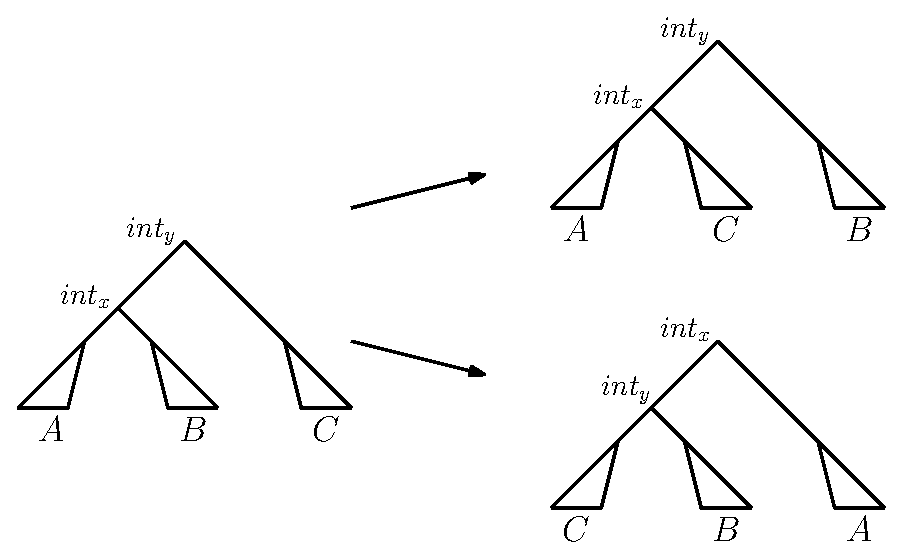
\includegraphics[width=0.7\textwidth]{nni_moves_internal_label}
% 		\caption{Two possible $\nni$ moves on edge $(int_x, int_y)$ where $x \in A, y \in B$.
% 		}
% 		\label{fig:nni_moves}
% 	\end{figure}
%
% 	The nodes incident to the edge after the $\nni$ move are labelled by $int_x$ and $int_y$ as well.
% 	By default, the node that has lower rank than the other one is labelled by $int_x$, the other one by $int_y$.
% 	But if $int_x$ is no ancestor of $x$ or $int_y$ is no ancestor of $y$, we swap the labels of the two new nodes, such that $\rank(int_x) > \rank(int_y)$.
% 	An example of an $\nni$ move and the new labelling is provided in Figure~\ref{fig:nni_example_internal_label}.
%
% 	\begin{figure}[H]
% 		\centering
% 		\includegraphics[width=0.8\textwidth]{nni_example_internal_label}
% 		\caption{The first labelling after the $\nni$ move preserves the ranks of $int_4$ and $int_6$.
% 		But then $int_6$ is not an ancestor of $6$ any more.
% 		Therefore, $int_4$ and $int_6$ have to change their labels.
% 		}
% 		\label{fig:nni_example_internal_label}
% 	\end{figure}
%
% 	We proceed to show that $int_x$ and $int_y$ are ancestors of $x$ and $y$ after an $\nni$ move as described above, respectively.
% 	If $x$ stays in the subtree rooted in the lower node of $e$, this does obviously hold.
% 	We now turn to the case that $x$ is not in the subtree rooted in the lower node of $e$ after the $\nni$ move.
% 	Then the labels of the two internal nodes change such that $\rank(int_x) > \rank(int_y)$.
% 	This makes sure that $int_x$ is an ancestor of $x$.
% 	Thus, it remains to prove that $int_y$ is ancestor of $y$.
% 	In particular, we need to show that $y$ is not in the same subtree $A$ as $x$, whose root has the node labelled by $int_x$ as parent before and after the $\nni$ move.
% 	Let us consider the tree before the $\nni$ move.
% 	$A$ has $|A|$ leaves and $|A| - 1$ internal nodes.
% 	These internal nodes are labelled by some leaves of $A$, because all internal nodes must be labelled by a descendant leaf.
% 	We know that $x \in A$, and the parent of the root of $A$ is labelled by $x$.
% 	All remaining $|A|-1$ leaf labels of $A$ appear as labels of the $|A|-1$ internal nodes of $A$.
% 	From the fact that the internal node labelled by $y$ is not inside $A$ we can conclude that $y$ cannot be a leaf of $A$.
% 	This proves that the labelling of the internal nodes is is well defined and allows a unique identification of internal nodes by their labels.
%
% 	The task is now to prove that there is always a caterpillar path at least as short as the given path $p$.
% 	Therefore, we use the following observation:
% 	Within each $\rnni$ move the ranks of at most two internal nodes change by at most one each.
% 	This is true for both rank moves and $\nni$ moves, according to our definition of the labelling:
% 	Within a rank move two nodes exchange their ranks, while there are not necessarily changes of ranks when $\nni$ moves are performed.
%
% 	On a caterpillar path the only possible moves are $\nni$ moves that change the ranks of two internal nodes by one each.
% 	Therefore, we can construct a caterpillar path $r$ out of $p$:
% 	every time two internal nodes $int_x$ and $int_y$ exchange ranks on $p$, they do so on the caterpillar path $r$ as well.
% 	Since there are moves on $p$ that do not change the ranks of internal nodes, this caterpillar path has length $|r| \leq |p|$.
% 	Hence, there is always a shortest path between $T$ and $R$ that is a caterpillar path.
% \end{proof}

\subsection{Split Theorem}
\label{section:split_theorem}
\todo{Split or Cluster?}

Within this section we will make a further step towards understanding the complexity of computing shortest paths in $\rnni$.
Since the problem of computing distances in the most common tree spaces as $\nni$ \autocite{Dasgupta2000-xa}, rooted $\spr$ \autocite{Bordewich2005-nx}, or $\tbr$ \autocite{Allen2001-ky} is known to be $\np$-hard, it is desirable to find a tree space that is less complex.
So far it is not known whether computing distances in $\rnni$ is $\np$-hard or not.
The natural approach to solve this question is to compare $\rnni$ and $\nni$ graph to see whether the proof of $\np$-hardness of $\nni$ can be transferred to $\rnni$.
Within this section we will explain why this is not the case.
Therefore we consider an example of shortest paths in $\nni$ that builds the key of the proof of its $\np$-hardness.
We will see that this example cannot be transferred to $\rnni$.
Following this, we will introduce the so-called Split Theorem, which generalises that example, and has been conjectured in \autocite{Gavryushkin2018-ol}.
However, we present a counterexample disproving the Split Theorem (Conjecture~\ref{conjecture:split_theorem}) in its original version and claiming the Cluster Theorem (Conjecture~\ref{conjecture:cluster_theorem}) as alternative version.

The proof of NP-completeness of $\nni$ in \autocite{Dasgupta2000-xa} is based on the fact that Theorem~\ref{thm:split_nni} holds for $\nni$.

\begin{theorem}
	There are trees $T,R$ in $\nni$ sharing a cluster which is not shared by any intermediate tree on any shortest path from $T$ to $R$.
	\label{thm:split_nni}
    %The formulation of this lemma is a bit different in Li1996-zw.
    %However, the lemma as stated here follows directly from Li1996-zw.
\end{theorem}

\begin{proof}
	See \autocite{Li1996-zw}.
\end{proof}

In the proof presented in \autocite{Li1996-zw} for Theorem~\ref{thm:split_nni} an example of two trees that share a cluster but have no shortest path that preserves this cluster is given.
The reason that this proof does not work for $\rnni$ is similar to the reason that caterpillar trees are convex in $\rnni$, but not in $\nni$.
Both trees $T$ and $R$ in the example of \autocite{Li1996-zw} have $2n$ taxa and consist of two caterpillar trees that share the root as parent.
The clusters given by the two nodes adjacent to the root are $\{1, \ldots, n\}$ and $\{n+1, \ldots, 2n\}$ in both trees $T$ and $R$.
There is a shortest path in $\nni$ where at first $T$ is transformed to a tree $T'$ with $n$ cherries where each cherry contains one taxon of $\{1, \ldots, n\}$ and one taxon of $\{n+1, \ldots, 2n\}$.
Afterwards, $T'$ is transformed to a tree $R'$ still containing the same cherries as $T'$ but in a way that resolving all these cherries of $R'$ results in $R$.
For proving that this path is shorter than any path preserving the clusters $\{1, \ldots, n\}$ and $\{n+1, \ldots, 2n\}$, the fact that $d_{\nni}(R,R') = d_{\nni}(T{\big|}_{\{1, \ldots, n\}}, R{\big|}_{\{1, \ldots, n\}})$ where $T{\big|}_{\{1, \ldots, n\}}$ and $R{\big|}_{\{1, \ldots, n\}}$ are $T$ and $R$ restricted to taxa $\{1,\ldots,n\}$, respectively, is being used.
However, this does not work in $\rnni$.
Similar to what we observed in the example depicted in Figure~\ref{fig:NNI_vs_RNNI}, there are lots of additional rank moves needed on a similar path in $\rnni$.
Therefore, a path where the two caterpillar trees are sorted separately, is shorter in $\rnni$.
\todo{(1) Do we want this explanation?
(2) If yes, is this explanation sufficient (we never say how we assign ranks to $T$ and $R$)?}



% \todo{Shall we keep this explanation? The problem is that the $\rnni$ path depends on the assignment of ranks to the cherries produced on the path}
% The counterexample presented in \autocite{Li1996-zw} works in $\nni$ because of the following:
% When proving Theorem~\ref{thm:split_nni}, \autocite{Li1996-zw} gives an example of two trees $T$ and $R$ on $2n$ taxa that consist of two caterpillar trees each that share the root as parent.
% The clusters given by the two nodes adjacent to the root are $\{1, \ldots, n\}$ and $\{n+1, \ldots, 2n\}$ in both trees $T$ and $R$.
% Between these there is a shortest path in $\nni$ where at first $T$ is transformed to a tree $T'$ with $n$ cherries where each cherry contains one taxon of $\{1, \ldots, n\}$ and one taxon of $\{n+1, \ldots, 2n\}$.
% Afterwards, $T'$ is transformed to a tree $R'$ still containing the same cherries as $T'$ but in a way that resolving all these cherries of $R'$ results in $R$.
% For proving that this path is shorter than any path preserving the clusters $\{1, \ldots, n\}$ and $\{n+1, \ldots, 2n\}$, the fact that $d_{\nni}(R,R') = d_{\nni}(T{\big|}_{\{1, \ldots, n\}}, R{\big|}_{\{1, \ldots, n\}})$ where $T{\big|}_{\{1, \ldots, n\}}$ and $R{\big|}_{\{1, \ldots, n\}}$ are $T$ and $R$ restricted to taxa $\{1,\ldots,n\}$, respectively, is being used.
% However, this does not work in $\rnni$.
% Introducing new cherries means introducing new internal nodes with new ranks.
% Since there are lots of rank moves needed for an $\rnni$ path similar to the shortest $\nni$ path presented above, the path in $\rnni$ that breaks the clusters $\{1, \ldots, n\}$ and $\{n+1, \ldots, 2n\}$ is no shortest path.

% ^How do we assign ranks to the new cherry nodes?
% We could either create a path where $R$ and $R'$ have distance equal to $d_{\rnni}(T{\big|}_{\{1, \ldots, n\}}, R{\big|}_{\{n+1, \ldots, 2n\}})$ and have a lot of additional rank moves before and after that part OR
% Build $R$ and $R'$ that contain all the cherries within the least number of moves possible (3n-3) and having a longer path between $R$ and $R'$.
% Also anything in between these two options is possible. Are we able to disprove every option??


Since the example given in \autocite{Li1996-zw} that proves Theorem~\ref{thm:split_nni} in $\nni$ does not work in $\rnni$, a contrary statement was conjectured in \autocite{Gavryushkin2018-ol}.
For understanding this conjecture it is important to realise the connection between edges in a tree and so-called splits, which are bipartitions of the taxon set of that tree:
By deleting an edge $e$ of a tree $T$ one receives two trees on taxon sets $A$ and $B$ such that $\{A,B\}$ is a partition of the taxon set of $T$.
Note that each edge induces such a bipartition, often written as $A|B$, and that both edges incident to the root of a tree induce the same partition.
Since these partitions are commonly referred to as \emph{splits}, the following conjecture was named \emph{Split Theorem} in \autocite{Gavryushkin2018-ol}.

\begin{conjecture}[Split Theorem]
	For the $\rnni$ graph the following statement holds:
	If a partition of leaves given by an edge is present in two trees $T$ and $R$ then the partition is presented in every tree on every shortest path between $T$ and $R$.
	\label{conjecture:split_theorem}
\end{conjecture}

However, we found a simple counterexample to this conjecture, provided in Figure~\ref{fig:splitthm_counterexample}.

\begin{figure}[H]
	\centering
	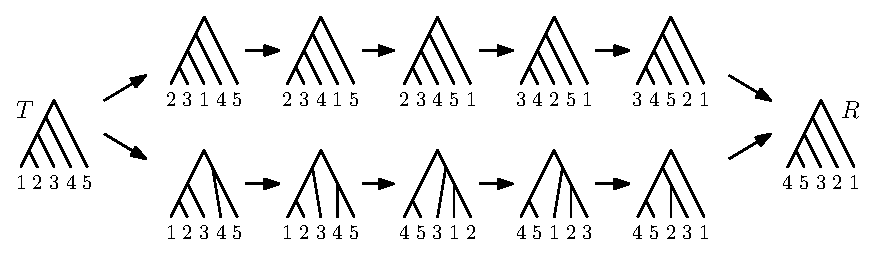
\includegraphics[width=\textwidth]{splitthm_counterexample}
	\caption{The split $123|45$ is present in $T$ and $R$, but the path at the top is a shortest path where none of the trees contains this split.
    However, this split is maintained on the path at the bottom, which is a shortest path as well.}
	\label{fig:splitthm_counterexample}
\end{figure}

Since the counterexample in Figure~\ref{fig:splitthm_counterexample} shows that the version of the Split Theorem stated in \autocite{Gavryushkin2018-ol} does not hold, we will now claim an alternative to this conjecture, the \emph{Cluster Theorem} (Conjecture~\ref{conjecture:cluster_theorem}).
Within the Cluster Theorem we are considering clusters instead of splits.
This is motivated by the fact that rooted phylogenetic trees can uniquely be represented by sets of clusters \autocite{Steel2016-ye}, but not by sets of splits as they cannot define the position of the root.
Moreover, a ranked tree can be uniquely determined by ordering the clusters such that the ranks of the internal nodes inducing those clusters increase.

% \begin{conjecture}[Weak Split Theorem]
% 	For $\rnni$ graph the following statement holds:
% 	if a partition of leaves given by an edge is present in two trees $T$ and $R$ then there exists a shortest path between $T$ and $R$ where this partition is present in every tree on this path.
% 	\label{split_theorem_weak}
% \end{conjecture}
%
% \todo{Do we want to keep the weak version of the split thm? It is stronger than the Cluster Thm!}
%
% The weak Split Theorem (in the version as in Lena's thesis) is computationally proven to hold for trees with up to $6$ taxa ($\sim 38$ min running time on laptop).

\begin{conjecture}[Cluster Theorem]
	For the $\rnni$ graph the following statement holds:
	if two trees $T$ and $R$ contain the same cluster $C$, then $C$ is present as cluster in every tree on every shortest path between $T$ and $R$.
	\label{conjecture:cluster_theorem}
\end{conjecture}

Note that trees $T$ and $R$ of counterexample~\ref{fig:splitthm_counterexample} induce the same set of splits, but have distinct clusters.
Furthermore, this counterexample can be used to prove that the Cluster Theorem does not hold in $\nni$.

\todo{LC: connect previous with following (has been in computation section before)}

%TODO
%How much detail do we need? Shall we have this as separate section or is it sufficient to mention that we checked the cluster theorem for up to $k$ taxa?

For proving the Cluster Theorem as stated in Conjecture~\ref{conjecture:cluster_theorem} for small trees, we implemented the algorithm for computing the $\rnni$ graph as stated above.
If the graph is computed, one can get distances by using algorithms such as Floyd-Warshall~\autocite{Floyd1962-ew} or Dijkstra~\autocite{Dijkstra1959-ph}.
However, the large number of vertices in $\rnni$ is an obstacle when it comes to computing distances.
For instance the Floyd-Warshall algorithm needs to save a matrix containing all pairwise distances of vertices in the graph, which needs space quadratic in the number of vertices.
Since there are $\frac{n!(n-1)!}{2^{n-1}}$ vertices in the $\rnni$ graph~\autocite{Gavryushkin2018-ol}, we already run out of space when considering $7$ taxa.
Therefore, we cannot simply use this algorithm to compute all distances in $\rnni$.
Instead of this we compute distances between certain pairs of trees and use the symmetry of $\rnni$ to draw conclusions about the remaining distances.

In the following we describe how the Cluster Theorem has computationally been proven for small trees.
For this aim only a restricted subset of trees in $\rnni$ needs to be considered, that is trees that share a cluster.
Furthermore, it is sufficient to consider clusters of the shape $\{1, \ldots, m\}$ for $2 \leq m \leq n-1$.
This is due to the fact that the distance $d(T_1,R_2)$ and $d(T_2,R_2)$ between two pairs of trees $(T_1,R_1)$ and $(T_2,R_2)$ are equal if one can receive $T_2$ from $T_1$ by permuting the taxa the same way as it is necessary for receiving $R_2$ from $R_1$.
Therefore, we compute for all $m = 2, \ldots, n-1$ exact $\rnni$ distances between all trees containing the cluster $\{1, \ldots, m\}$, using Dijkstra.
Additionally, the subgraph of $\rnni$ only consisting of trees that have $\{1, \ldots, m\}$ as cluster is computed.
All pairwise distances between the trees in the subgraph are computed, by using Floyd-Warshall, to compare them with the distances in $\rnni$.
With this approach it is possible to show that the Cluster Theorem holds for up to $6$ taxa. \todo{Can we improve this?}

\section{Ideas}
\todo{This section is just a rough draft. Are there ideas we want to keep? Shall this become an 'open problems/future work' section?}


The paths computed by $\findpath$ depend on the order of input trees $T$ and $R$:
$\findpath(T,R)$ does not necessarily produce the reverse path of $\findpath(R,T)$.
An example can be found in Figure~\ref{fig:findpath_not_symmetric}.
However, simulations suggest that the lengths of the two paths computed by $\findpath$ for one pair of trees are equal.

\begin{conjecture}
    Let $T$ and $R$ be ranked trees.
    The lengths of paths $\findpath(T,R)$ and $\findpath(R,T)$ are equal.
\end{conjecture}

\begin{figure}[H]
	\centering
	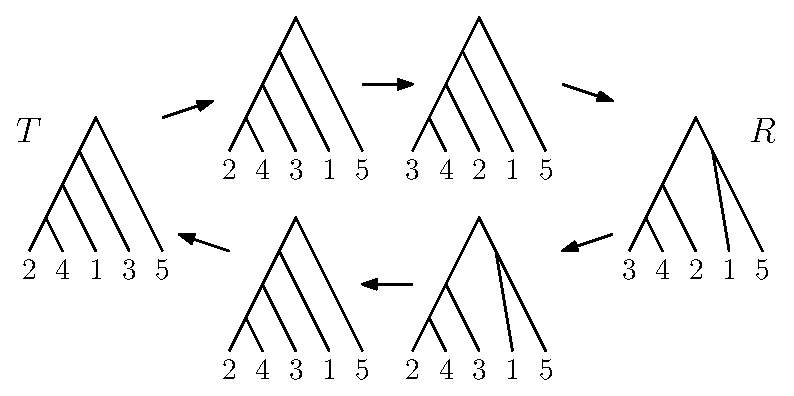
\includegraphics[width=0.7\textwidth]{findpath_not_symmetric}
	\caption{Two paths computed by $\findpath$. At the top $\findpath(T,R)$, at the bottom $\findpath(R,T)$}
	\label{fig:findpath_not_symmetric}
\end{figure}

% idea for description of max distance caterpillar trees:
\begin{lemma}
    Let $T$ and $R$ be caterpillar trees.
    It is $d_c(T,R) = \Delta(\rnni)$ if, and only if, $T$ and $R$ share no induced triplet.
    \todo{define induced triplets}
\end{lemma}

This Lemma does only hold for caterpillar trees and not for trees with more than one cherry.
Furthermore, triplets do not represent ranked trees uniquely as they do not contain information about the ranks of internal nodes (but they can uniquely define caterpillar trees as these only have one cherry)

\begin{proof}
    %TODO
    % Insert the proof here
    Fix $T = (\ldots(1,2) \ldots ,n)$, use induction on $n$ and $\csort$ (taxon $n$ must be in cherry of $R$ if distance is max).
\end{proof}

According to Algorithm~\ref{alg:max_dist_tree}, the number of trees with maximum distance to a given caterpillar tree $T$ is $(n-1)!$.
The number of caterpillar trees with distance $\Delta(\rnni)$ from a given caterpillar tree is $2^{n-2}$.


\subsection{Partition lattice}

% Define Partition Lattice $\Pi_n$ and max chains in that lattice!

\begin{theorem}
The $\rnni$ graph on $n$ taxa is isomorphic to the graph of maximal chains of the partition lattice $\Pi_n$ where two maximal chains are connected by an edge if and only if they differ by exactly one partition.
The corresponding metric spaces are isometric.
\end{theorem}


\printbibliography

\end{document}
